\lecture{4}{Jan 24 01:10}{}
\section{Infintie Potential Square Well}
\begin{remark}
    \begin{figure}[H]
        \centering
        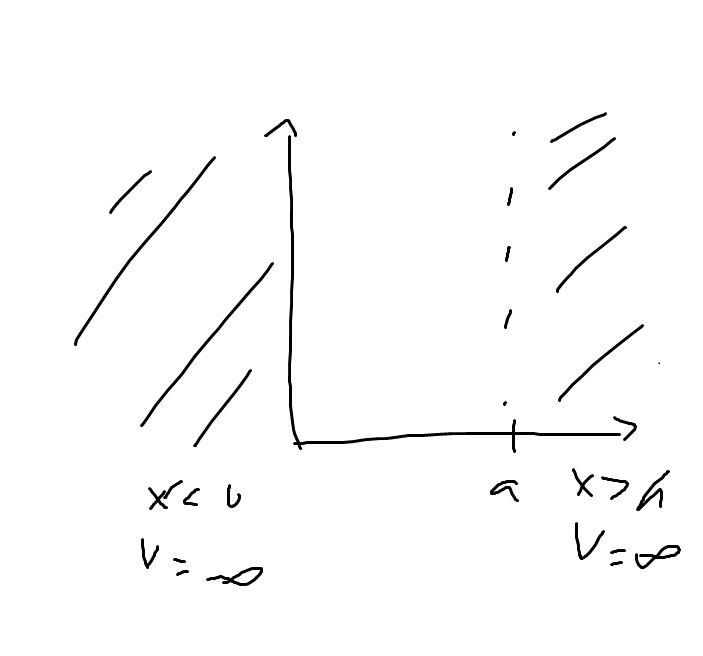
\includegraphics[width=0.8\textwidth]{Figures/02.png}
        \caption{}
        \label{fig:}
    \end{figure}
    Classically what we would see is a particle going back and forth in the square well. If we take a snapshot in time, 
    there would be an equal probability being anywhere (not really but roughly speaking). In the classic case, we recall 
    that the energy states of the first energy level was 
    \[
        \psi  = \sin (\pi \frac{x}{a})
    \]
    as shown in Figure 1.2 and the probability would be 
    \[
        \vert \psi _1 \vert ^{2}  =\alpha ^{2}  \sin  ^{2}  (\pi \frac{x}{a})
    \]
    The next solution we have is where \(n =2 \),  \(\psi  = \alpha  \sin  (2\pi \frac{x}{a})\) and we can observe 
    where the function goes to 0. 
    \[
        \psi _n (x) = \sqrt{\frac{2}{a}} \sin (n \pi \frac{x}{a}), A = \sqrt{\frac{2}{a}} 
    \]
    \[
         1 = A ^{2}  \int_0^a  \mathrm{d}x \vert \psi _n(x) \vert ^{2} 
    \]
    where we can determine the normalization factor from here. 
\end{remark}
\begin{remark}
The superposition we want to consider now is 
    \[
        \psi (x, 0) = \frac{1}{\sqrt{2} } \left[ \psi _1 + \psi _2 \right] 
    \]
    Now we are determing the expectation value of the energy \(\langle E \rangle \) 
    \[
        \int_{0}^{x} \psi ^* \hat{H} \psi  \,\mathrm{d}x 
    \] note that applying the Hamiltonian operator is applied on the real operator as when operating on the first complex factor 
    gives a different result. We see that 
    \[
        \psi _n ^* = \psi _n \implies \psi = \psi ^*
    \]
    Thus we can write that 
    \[
        \langle E \rangle = \int_{0}^{a}  \hat{H} \psi \psi \,\mathrm{d}x 
    \]
    We now basically have the answer where 
    \[
        \langle \hat{H}  \rangle = \int_{0}^{a}  (\hat{H} \psi ) \psi \,\mathrm{d}x 
    \]
    \[
        =\frac{1}{2} \int_{0}^{a}  \left[ \hat{H} (\psi _1 + \psi _2) \right] (\psi _1 +\psi _2) \,\mathrm{d}x 
    \]
    \[
        =\frac{1}{2} \int_{0}^{a}  \left[ E_1\psi _1 + E_2 \psi _2  \right](\psi _1+\psi _2) \,\mathrm{d}x 
    \]
    \[
        =\frac{1}{2} \int_{0}^{a} \left[ E_1 \psi _1 ^{2}  + E_1 \psi _1 \psi _2 +E_2 \psi _1 \psi _2 + E_2 \psi _2 ^{2}  \right]   \,\mathrm{d}x 
    \]
    \[
        = \frac{1}{2}\left( E_1 + E_2 \right) \int_{0}^{a} \psi _1 \psi _2 (E_1 + E_2)  \,\mathrm{d}x 
    \]
    Now we wish to consider the generic case 
    \[
        \int_{0}^{a}  \psi _m \psi _ n\,\mathrm{d}x 
    \]
    \[
        = \int_{0}^{a}\frac{2}{a} \sin (m \pi \frac{x}{a}) \sin (n \pi  \frac{x}{a})  \,\mathrm{d}x 
    \]
    \[
        = \frac{2}{a} \int_{0}^{a} \left[ \cos (\frac{m-n}{a} \pi x) - \cos (\frac{m+n}{a}\pi x) \right]   \,\mathrm{d}x 
    \]
    \[
        =\frac{2}{a} \at{\left[ \frac{a}{(m-n)\pi }\sin (\frac{m-n}{a} \pi x) - \frac{a}{(m+n) \pi } \sin (\frac{m+n}{a}\pi x) \right] }{0}{a} 
    \]
    \[
        =0 , m\neq  n
    \]
    To summarize, we have shown that 
    \[
        \int_{0}^{a} \psi _n \psi _m  \,\mathrm{d}x =  \begin{dcases}
            1, &\text{ if } m=n  ;\\
            0, &\text{ if } m \neq  n;\\
        \end{dcases} = \delta_{mn} 
    \]
    therefore the cross terms must go away and will be just the average value. 
\end{remark}
\begin{remark}
    Time Dependence: 
    \[
        \psi _n (x,t) =\sqrt{\frac{2}{a}} \sin (n \pi \frac{x}{a})e^{-i \frac{E_n}{\hbar }t}
    \]
    What does our superposition look like:
    \[
        \psi  = \frac{1}{\sqrt{2} } \left[ \psi _1 + \psi_2 \right] = \frac{1}{\sqrt{2} } \left[ \psi _1 e^{-i \frac{E_1}{\hbar}t} + \psi _2 e^{-i \frac{E_2}{\hbar }t}  \right] 
    \]
    \[
        \langle \hat{H}  \rangle = \frac{1}{2} \int_{0}^{a}  (\hat{H} \psi^* )\psi \,\mathrm{d}x 
    \] Note that we can no longer ignore the complex conjugate term and compute the quantity 
    \[
        \langle \hat{H}  \rangle = \frac{1}{2} \int_{0}^{a} \left[ \hat{H} \left( \psi _1 e^{\frac{iE_1}{\hbar }t} + \psi _2 e^{\frac{iE_2}{\hbar }t}   \right)  \right] \left( \psi _1 e^{-\frac{iE_1}{\hbar }t} + \psi _2 e^{-\frac{iE_2}{\hbar }t}   \right)    \,\mathrm{d}x 
    \]
    \[
        = \frac{1}{2} \int_{0}^{a} \left[  E_1 \psi _1 e^{i \omega _1 t} + E_2 \psi _2 e^{i \omega _2 t} \right] \left[ \psi _1 e^{-i \omega _1 t} + \psi _2 e^{-i \omega  _2 t} \right]   \,\mathrm{d}x 
    \]
    \[
        = \frac{1}{2 } \int_{0}^{a} \left[ E_1 \psi _1 ^{2}  + E_2 \psi _2 ^{2} + E_1 \psi _1 \psi _2 e^{i (\omega _1 - \omega _2)t} + E_2 \psi _1 \psi _2 e^{-i(\omega _1 - \omega _2)t} \right]   \,\mathrm{d}x 
    \]
    \[
         = \frac{1}{2} (E_1 + E_2 ) + \frac{1}{2}\int_{0}^{a} E_1 \psi _1 \psi _2 e^{i (\omega _1 - \omega _2)t} + E_2 \psi _1 \psi _2 e^{-i(\omega _1 - \omega _2)t}  \,\mathrm{d}x 
    \]
    \[
        =\frac{1}{2} (E_1 + E_2)
    \]
\end{remark}

\begin{remark}
    When we think about vector spaces we usually think of our own Euclidean space with three basis vectors that can create any vector in the subspace where 
    \[
        \vec{r}  = a \hat{x}  + b \hat{y} + c \hat{z} 
    \]
    or written as 
    \[
        \sum_{i=1}^3 \alpha_i \hat{x} _i 
    \]
    In principle, the superposition state is the sum of two basis functions. Thus, we can write down the wave function in two different ways:
    \[
        \psi  = \sum_{n=1}^{\infty} c_{n} \psi _n  
    \]
    now this is our vector spanned by our basis vectors \(\psi _n\)
    \[
        \begin{pmatrix}
             \frac{1}{\sqrt{2} } \\
              \frac{a}{\sqrt{2} }\\
              \frac{1}{\sqrt{2} }\\
              0\\
              \vdots \\
              0 \\
        \end{pmatrix}
    \] 
    Now we realize that quantum mechanics is just linear algebra where r
    \[
        \hat{H} _{\infty \times \infty } \vec{\psi}  = \vec{E} 
    \]
    Note that all must happen is that we satisfy the boundary conditions and end up with a DFT.
\end{remark}